\chapter{Results}

This chapter reports empirical outcomes under the protocol defined in Chapter \ref{chapter:experimental-design}. Both scenarios follow the same reporting structure and metric schema.

\section{Environment and Data Sanity Check}

Table~\ref{tab:ch8_sanity_profiles} verifies that profile scaling changes the realized trip intensity and decision density as intended. The mean trip count, variance, and Fano-like ratio increase from \textit{sparse} to \textit{dense}, and the number of decision transitions also grows accordingly.

\begin{table}[H]
\centering
\caption{Trip and decision-opportunity statistics by profile (Scenario~1 evaluation runs).}
\label{tab:ch8_sanity_profiles}
\begin{tabular}{lrrrr}
\toprule
Profile & Trip count mean & Trip count var & Fano-like & Mean transitions (ckpt) \\
\midrule
Sparse & 74.6550 & 78.3318 & 1.0493 & 0.9775 \\
Main   & 233.3450 & 325.4295 & 1.3946 & 3.9650 \\
Dense  & 360.8075 & 630.0957 & 1.7463 & 5.7100 \\
\bottomrule
\end{tabular}
\end{table}

These sanity checks support two points. First, the simulation is not operating at a single fixed demand level. Second, the RL policy is exposed to progressively denser decision opportunities under \textit{main} and \textit{dense}, which is necessary for observable learning effects.

\begin{figure}[H]
\centering
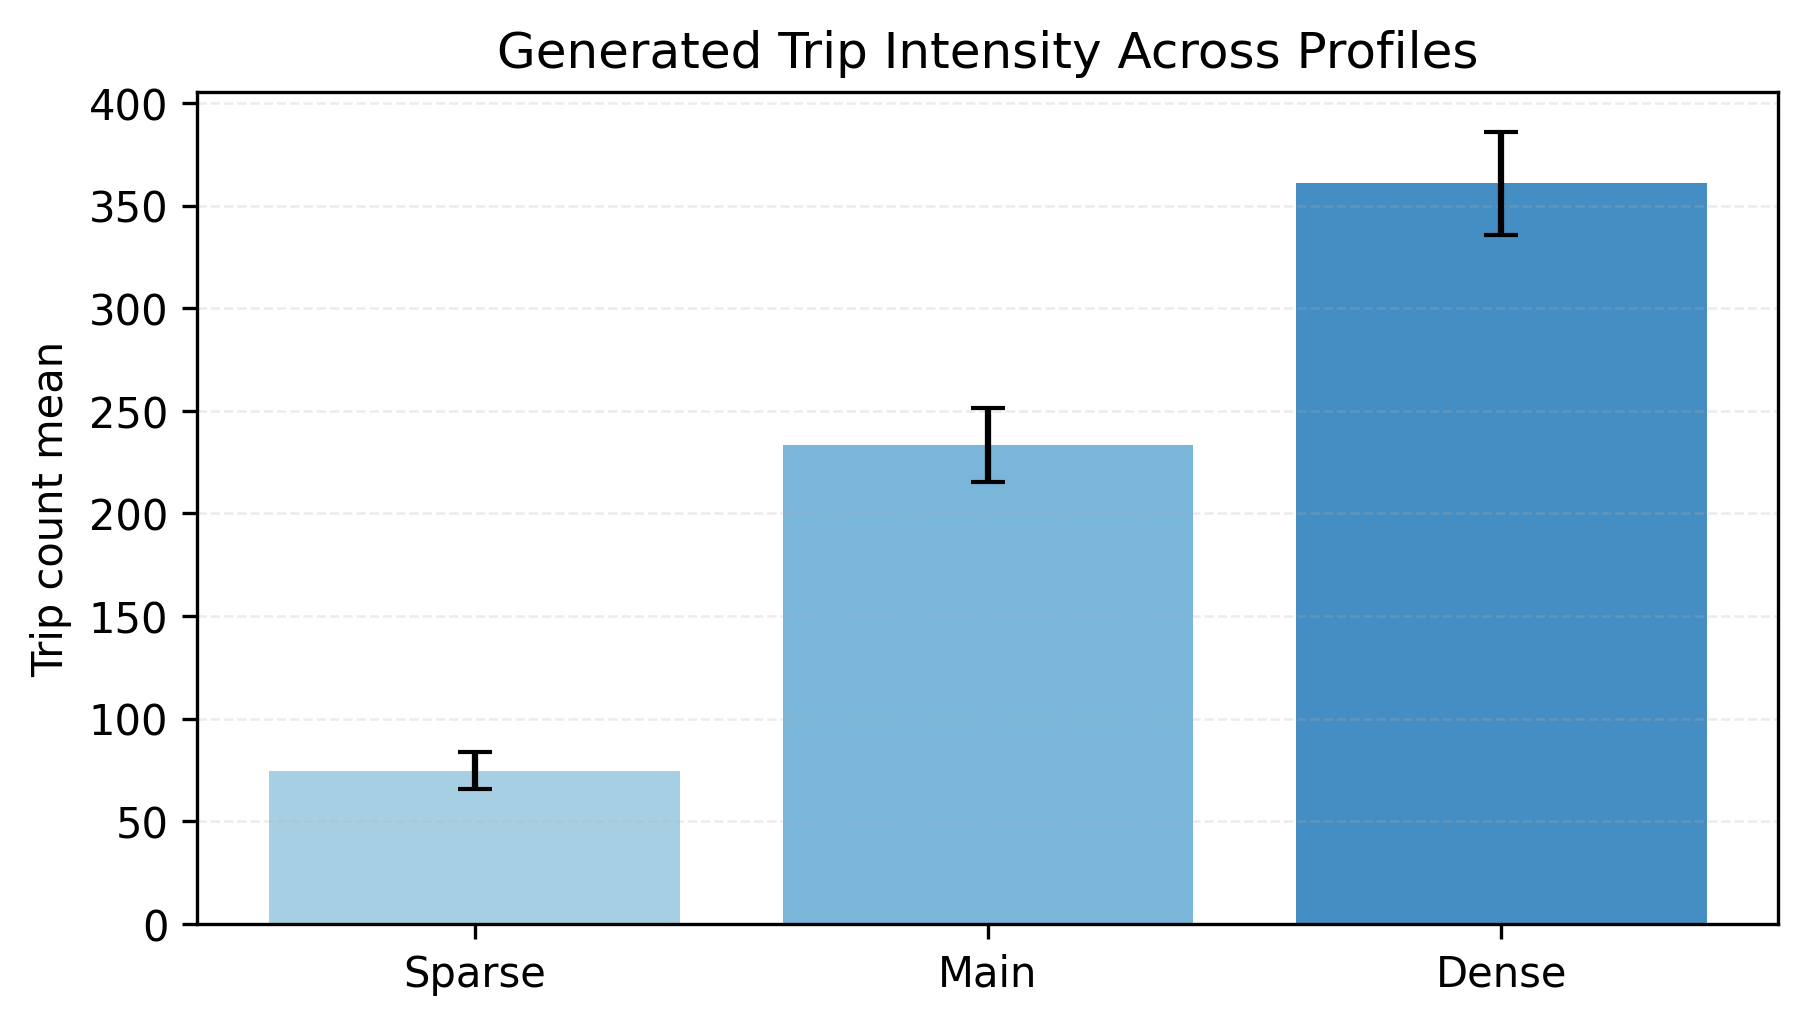
\includegraphics[width=0.86\textwidth]{figures/ch8_fig_6_2_generated_trip_intensity.png}
\caption{Generated trip intensity across sparse/main/dense profiles (error bars show one standard deviation from episode-level variance).}
\label{fig:ch8_trip_intensity_profiles}
\end{figure}

\begin{figure}[H]
\centering
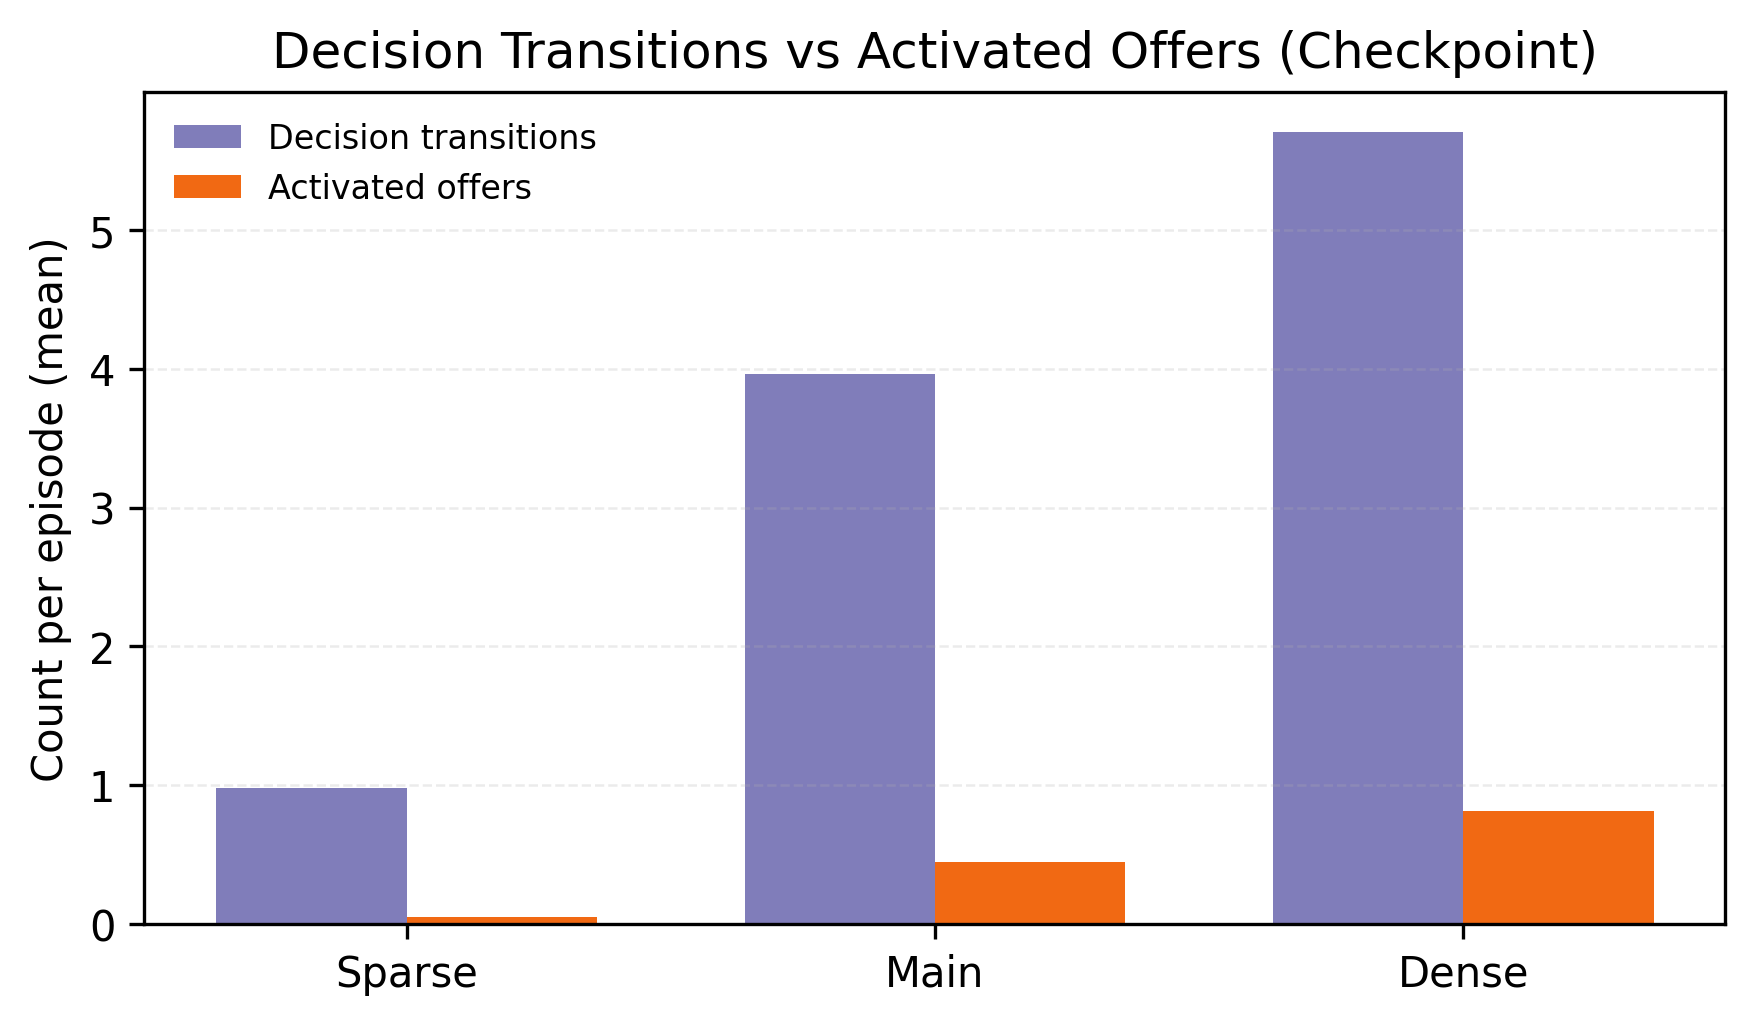
\includegraphics[width=0.86\textwidth]{figures/ch8_fig_6_3_offer_transition_density.png}
\caption{Decision transitions and activated offers across profiles under the checkpoint policy. Here, transitions denote RL state transitions (\(s,a,r,s',done\)); offers denote activated offers, not total offer opportunities.}
\label{fig:ch8_offer_transition_density}
\end{figure}

\section{Scenario 1 Results}

\subsection{Training Dynamics}

This subsection reports the learning dynamics of Scenario~1 under the final training protocol.

\begin{figure}[H]
\centering
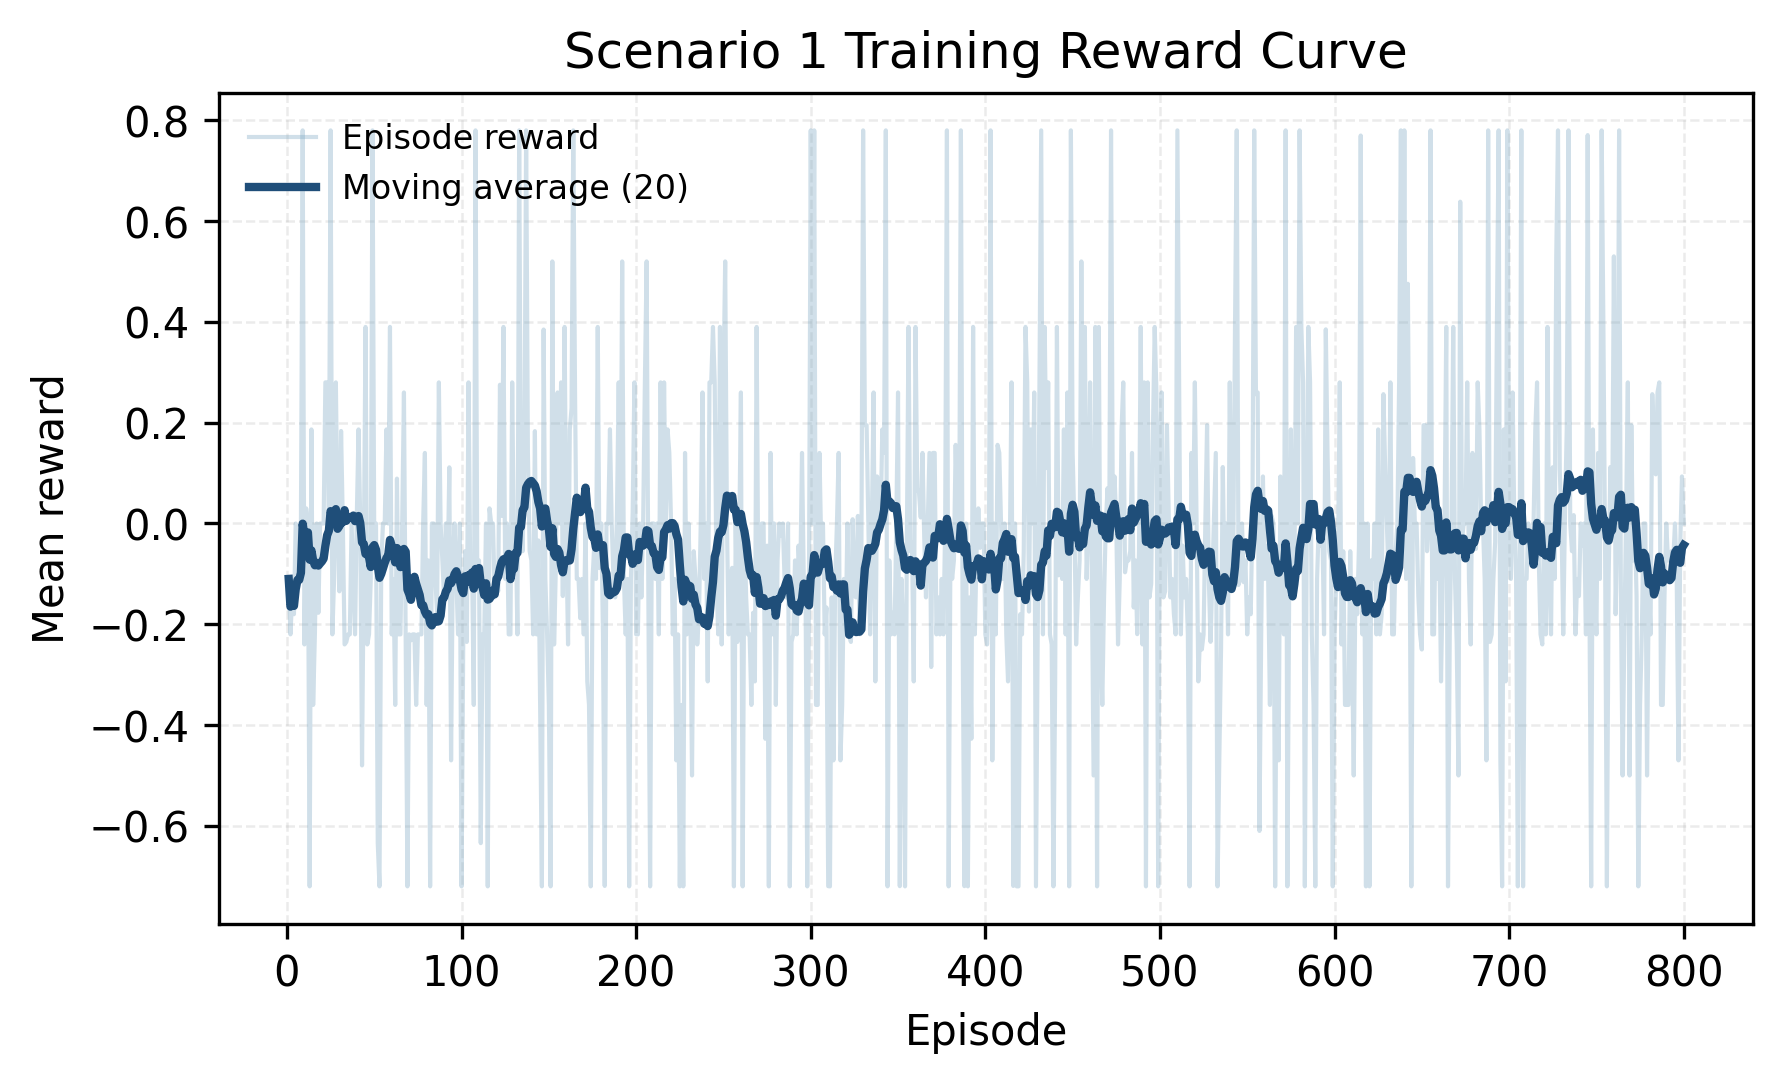
\includegraphics[width=0.9\textwidth]{figures/ch8_fig_6_4_s1_train_reward_curve.png}
\caption{Scenario~1 training reward curve (episode reward and moving average).}
\label{fig:ch8_s1_train_reward}
\end{figure}

\begin{figure}[H]
\centering
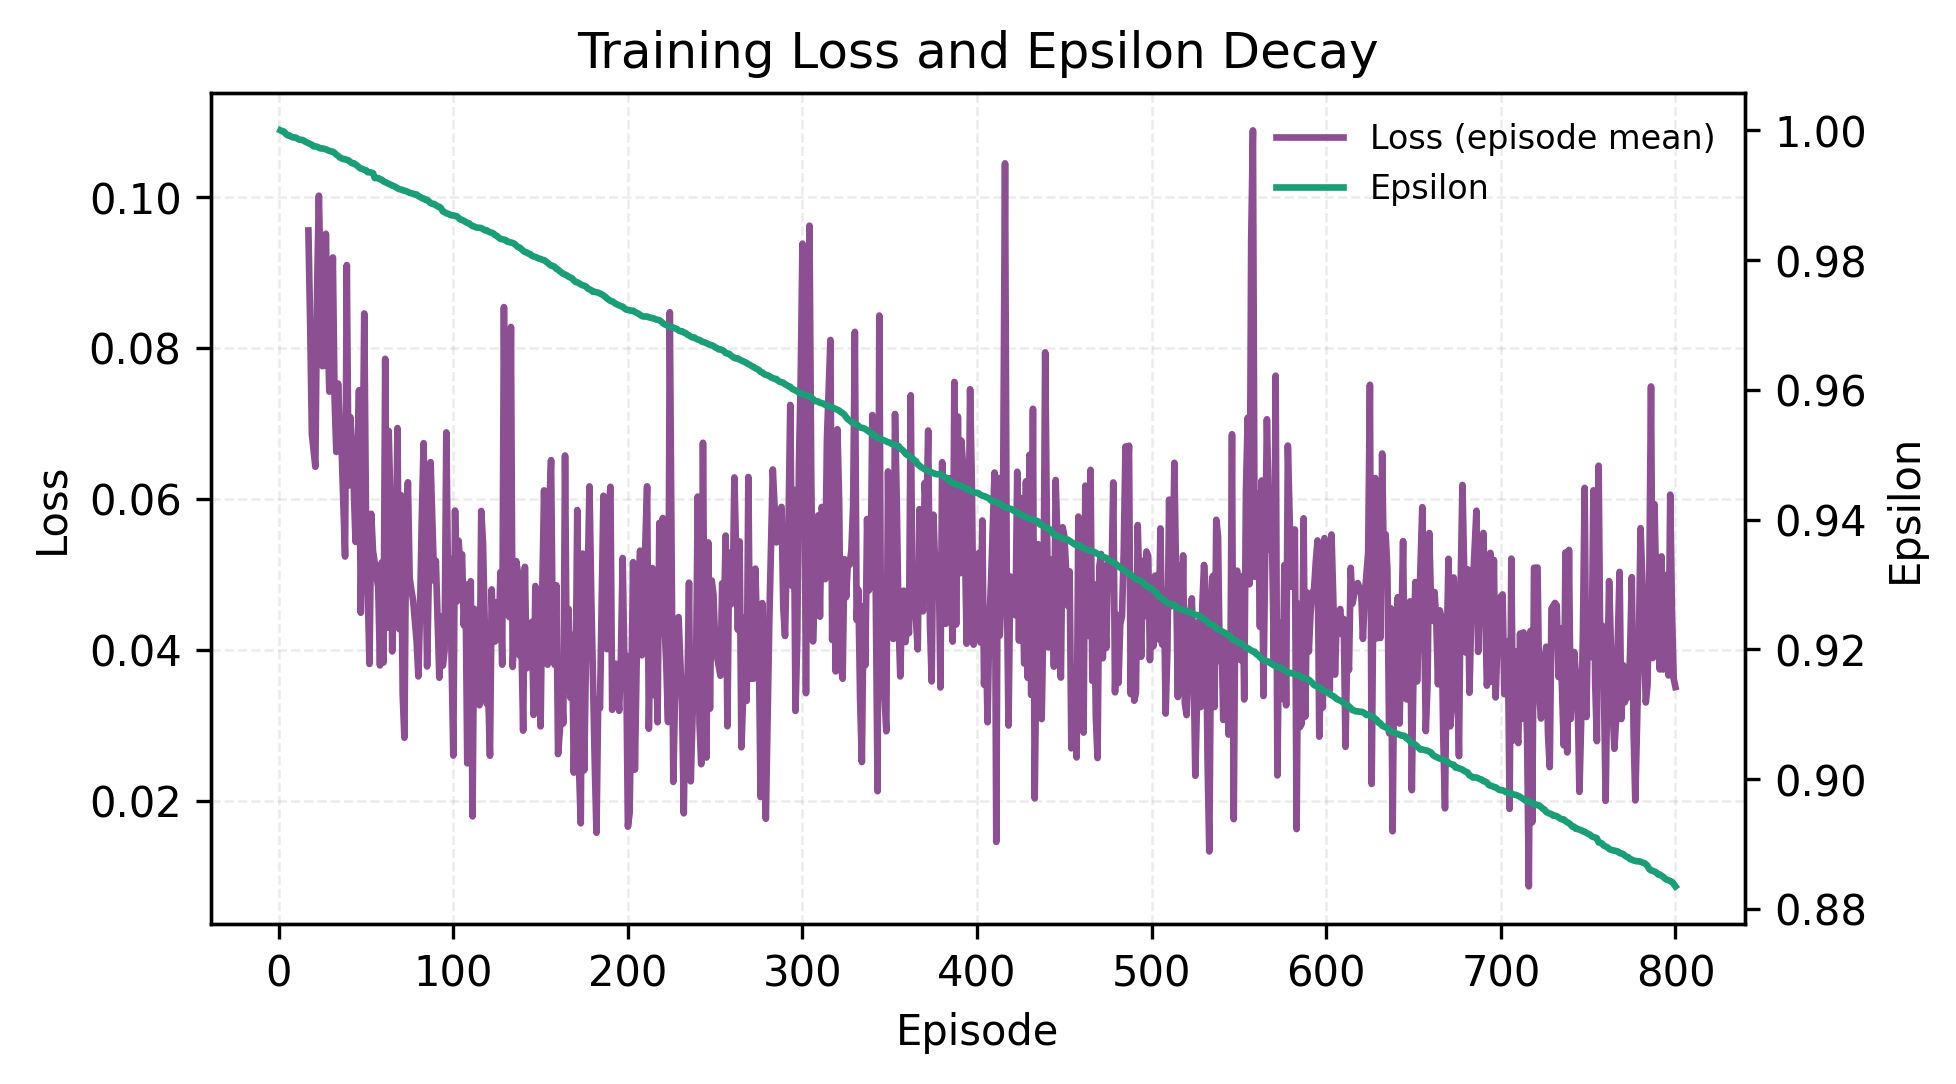
\includegraphics[width=0.9\textwidth]{figures/ch8_fig_6_5_s1_train_loss_epsilon.png}
\caption{Scenario~1 training loss and epsilon decay.}
\label{fig:ch8_s1_train_loss_epsilon}
\end{figure}

\begin{figure}[H]
\centering
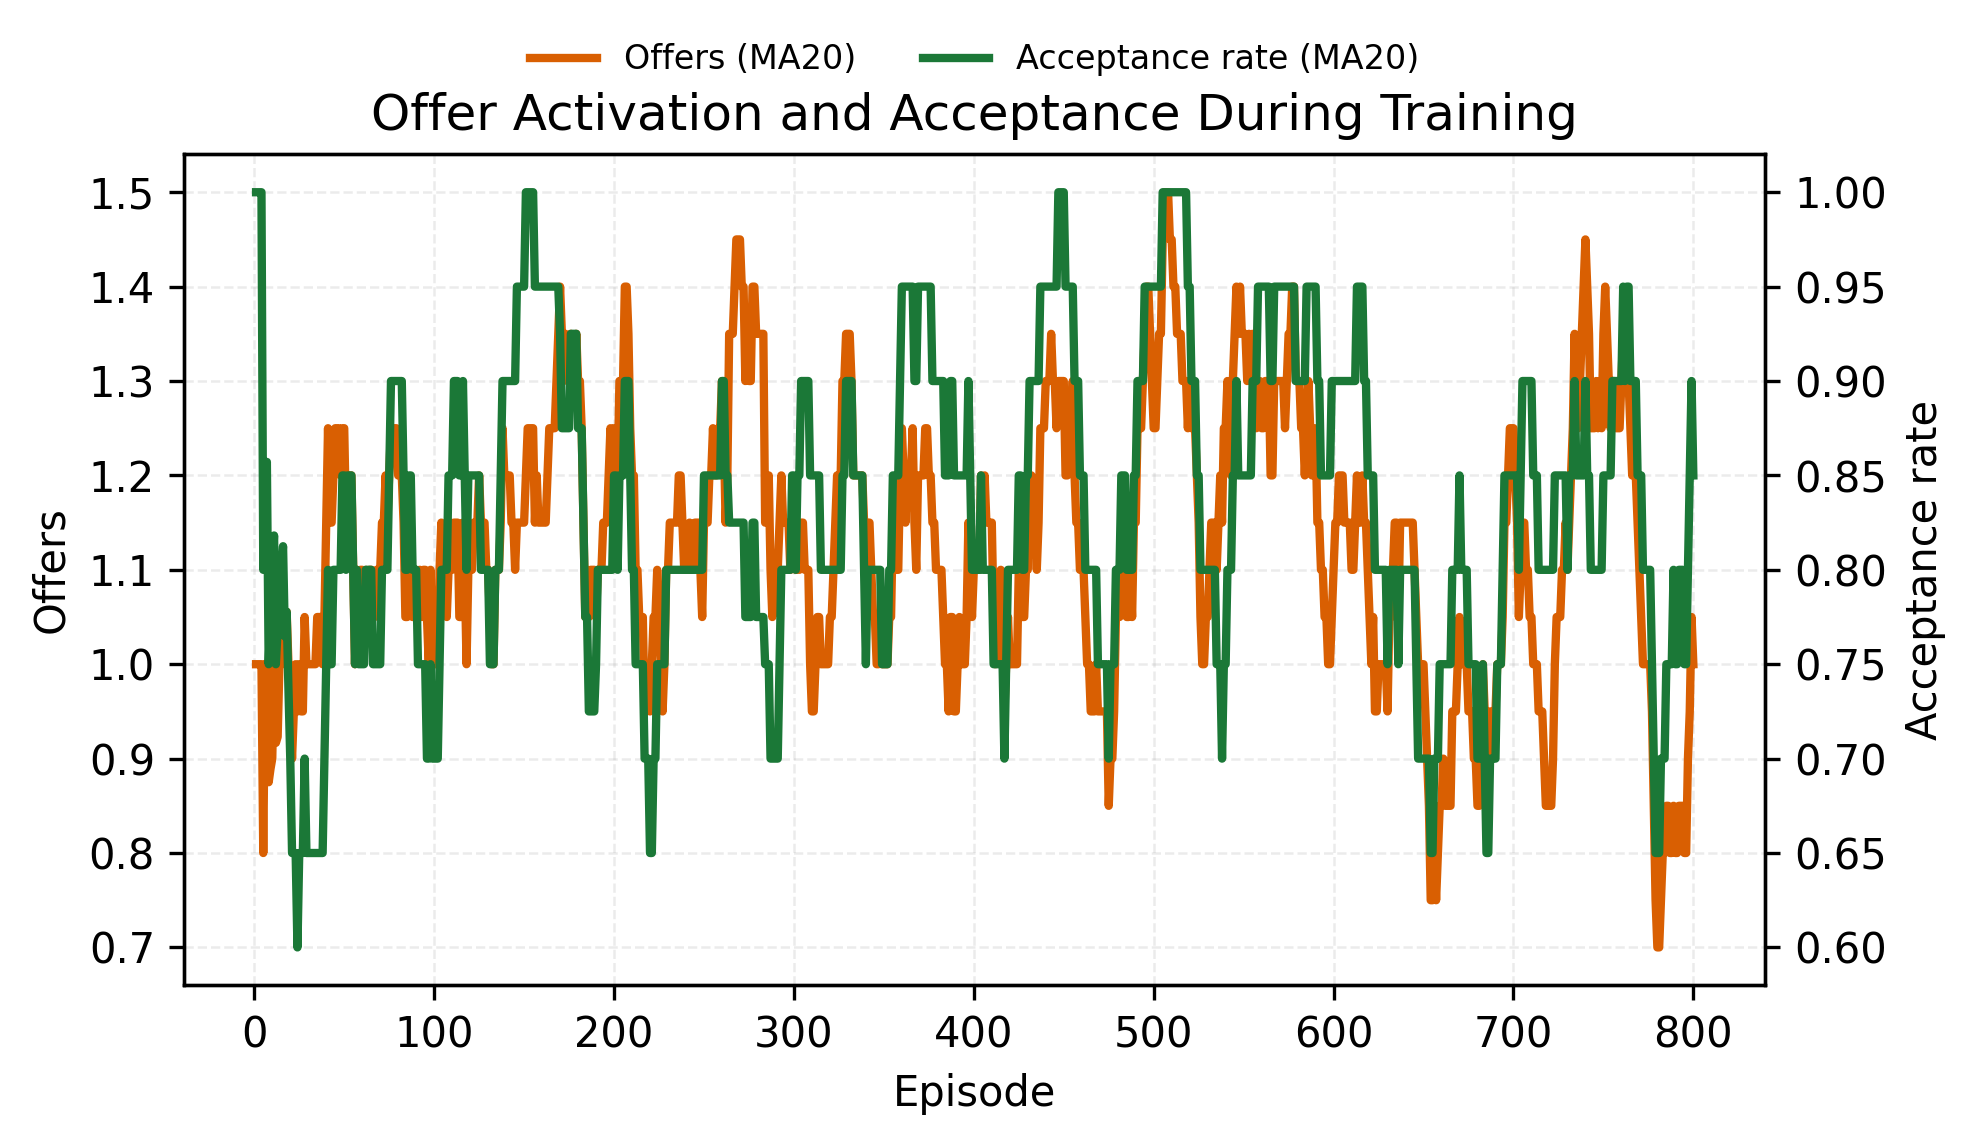
\includegraphics[width=0.9\textwidth]{figures/ch8_fig_6_6_s1_train_offers_acceptance.png}
\caption{Scenario~1 training offer activation and acceptance dynamics.}
\label{fig:ch8_s1_train_offer_accept}
\end{figure}

\begin{table}[H]
\centering
\caption{Scenario~1 training summary (last 100 episodes).}
\label{tab:ch8_s1_train_summary}
\begin{tabular}{lrrrrrr}
\toprule
Episodes & Mean reward & Std reward & Mean loss & $\epsilon_{end}$ & Mean offers & Mean accept rate \\
\midrule
100 & -0.0249 & 0.3171 & 0.0392 & 0.8835 & 1.0600 & 0.8200 \\
\bottomrule
\end{tabular}
\end{table}

Figures~\ref{fig:ch8_s1_train_reward}, \ref{fig:ch8_s1_train_loss_epsilon}, and \ref{fig:ch8_s1_train_offer_accept} show stable optimization with sustained policy activity. Table~\ref{tab:ch8_s1_train_summary} confirms that the late-stage training regime remains active and does not collapse to a trivial no-offer behavior.

\subsection{Main-Profile Policy Comparison}

Table~\ref{tab:ch8_main_policy} reports the primary comparison under the \textit{main} profile. Compared with fixed policies, the checkpoint policy achieves the highest mean reward while maintaining comparable service rate.

\begin{table}[H]
\centering
\caption{Main-profile policy comparison (Scenario~1).}
\label{tab:ch8_main_policy}
\small
\setlength{\tabcolsep}{4pt}
\resizebox{\textwidth}{!}{%
\begin{tabular}{lrrrrrrrr}
\toprule
Policy & Service rate (mean $\pm$ std) & Offers & Accepted & Acceptance rate & Mean reward (mean $\pm$ std) & Mean realized loss & Mean $\Delta EDL$ (mean $\pm$ std) & Mean transitions \\
\midrule
No-offer     & 0.9639 $\pm$ 0.0243 & 0.0225 & 0.0000 & 0.0000 $\pm$ 0.0000 & -0.0253 $\pm$ 0.0861 & 0.1667 & 0.0000 $\pm$ 0.0000 & 4.8725 \\
Always-offer & 0.9644 $\pm$ 0.0245 & 1.4625 & 1.4425 & 0.9157 $\pm$ 0.2750 & -0.0752 $\pm$ 0.4196 & 0.8425 & -0.1248 $\pm$ 0.1374 & 1.4425 \\
Checkpoint   & 0.9644 $\pm$ 0.0244 & 0.4475 & 0.4250 & 0.3779 $\pm$ 0.4851 & 0.1154 $\pm$ 0.2731 & 0.2854 & 0.0091 $\pm$ 0.0190 & 3.9650 \\
\bottomrule
\end{tabular}
}
\end{table}

Under the main profile, the checkpoint policy is more selective than \textit{always-offer} (fewer offers and fewer accepted relocations) and avoids its negative EDL trend. Relative to \textit{no-offer}, checkpoint activates additional offers and converts that activity into positive mean reward. Figure~\ref{fig:ch8_main_kpi_comparison} shows this policy separation visually.

\begin{figure}[H]
\centering
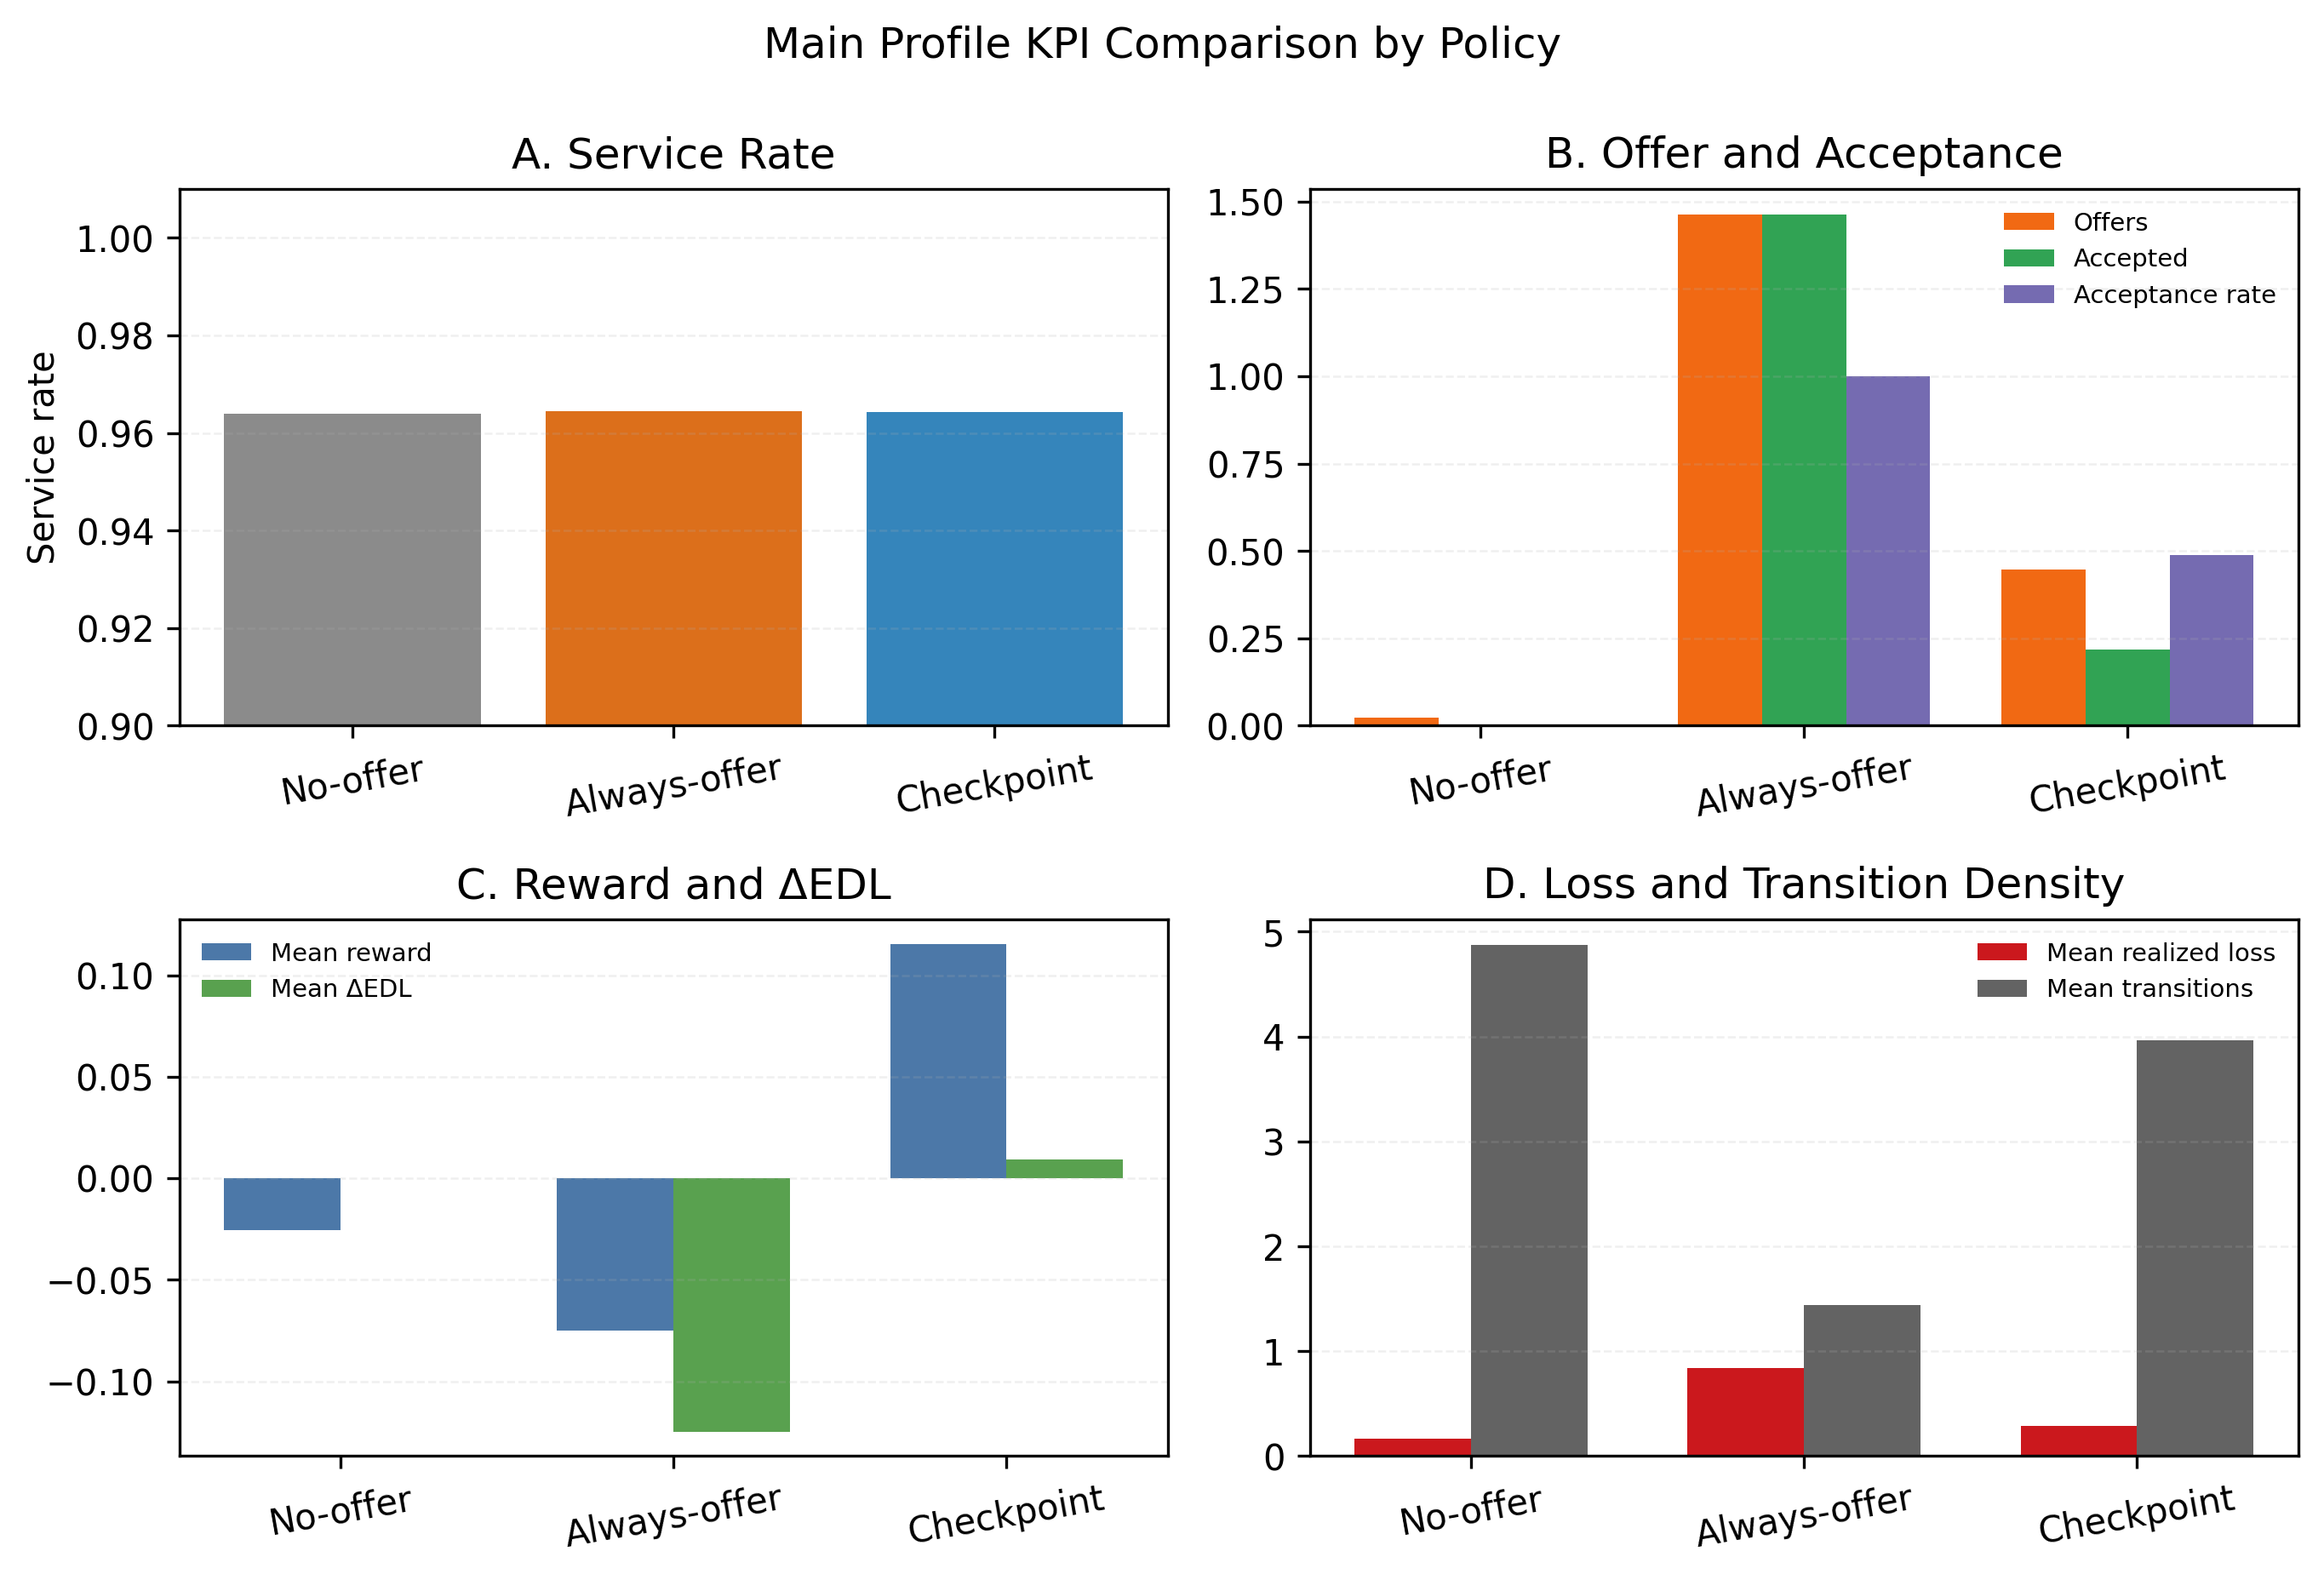
\includegraphics[width=0.9\textwidth]{figures/ch8_fig_6_7_main_profile_kpi_comparison.png}
\caption{Main-profile KPI comparison across no-offer, always-offer, and checkpoint policies (2x2 panel: service rate; offer/acceptance behavior; reward and $\Delta EDL$; realized-loss and transition density).}
\label{fig:ch8_main_kpi_comparison}
\end{figure}

\subsection{Robustness Across Sparse/Main/Dense Profiles}

Table~\ref{tab:ch8_robustness_three_profiles} summarizes the same policy trio across all three profiles.

\begin{table}[H]
\centering
\caption{Policy comparison across sparse/main/dense profiles (Scenario~1).}
\label{tab:ch8_robustness_three_profiles}
\small
\setlength{\tabcolsep}{4pt}
\resizebox{\textwidth}{!}{%
\begin{tabular}{llrrrrr}
\toprule
Profile & Policy & Service rate (mean $\pm$ std) & Offers & Mean reward (mean $\pm$ std) & Mean $\Delta EDL$ (mean $\pm$ std) & Mean realized loss \\
\midrule
Sparse & No-offer     & 0.9984 $\pm$ 0.0057 & 0.0000 & 0.0000 $\pm$ 0.0000  & 0.0000 $\pm$ 0.0000  & 0.0000 \\
Sparse & Always-offer & 0.9991 $\pm$ 0.0045 & 0.6600 & -0.0832 $\pm$ 0.1995 & -0.0929 $\pm$ 0.1160 & 0.0025 \\
Sparse & Checkpoint   & 0.9985 $\pm$ 0.0056 & 0.0525 & 0.0305 $\pm$ 0.1443  & 0.0016 $\pm$ 0.0082  & 0.0000 \\
\midrule
Main & No-offer       & 0.9639 $\pm$ 0.0243 & 0.0225 & -0.0253 $\pm$ 0.0861 & 0.0000 $\pm$ 0.0000  & 0.1667 \\
Main & Always-offer   & 0.9644 $\pm$ 0.0245 & 1.4625 & -0.0752 $\pm$ 0.4196 & -0.1248 $\pm$ 0.1374 & 0.8425 \\
Main & Checkpoint     & 0.9644 $\pm$ 0.0244 & 0.4475 & 0.1154 $\pm$ 0.2731  & 0.0091 $\pm$ 0.0190  & 0.2854 \\
\midrule
Dense & No-offer      & 0.9104 $\pm$ 0.0339 & 0.0450 & -0.0529 $\pm$ 0.0996 & 0.0000 $\pm$ 0.0000  & 0.6904 \\
Dense & Always-offer  & 0.9088 $\pm$ 0.0354 & 1.6925 & -0.1098 $\pm$ 0.4395 & -0.0938 $\pm$ 0.1288 & 4.2175 \\
Dense & Checkpoint    & 0.9100 $\pm$ 0.0346 & 0.8125 & 0.0971 $\pm$ 0.2649  & 0.0133 $\pm$ 0.0336  & 1.8940 \\
\bottomrule
\end{tabular}
}
\end{table}

Three robustness observations are consistent across profiles:
\begin{itemize}
\item checkpoint mean reward remains positive in all three profiles;
\item checkpoint mean $\Delta EDL$ remains positive, while \textit{always-offer} is negative;
\item checkpoint preserves service rate close to fixed-policy baselines without over-activating offers.
\end{itemize}

As shown in Figures~\ref{fig:ch8_reward_edl_robustness} and \ref{fig:ch8_offers_robustness}, seed-level dispersion increases from sparse to dense, which is consistent with stronger demand uncertainty under denser profile settings.

\begin{figure}[H]
\centering
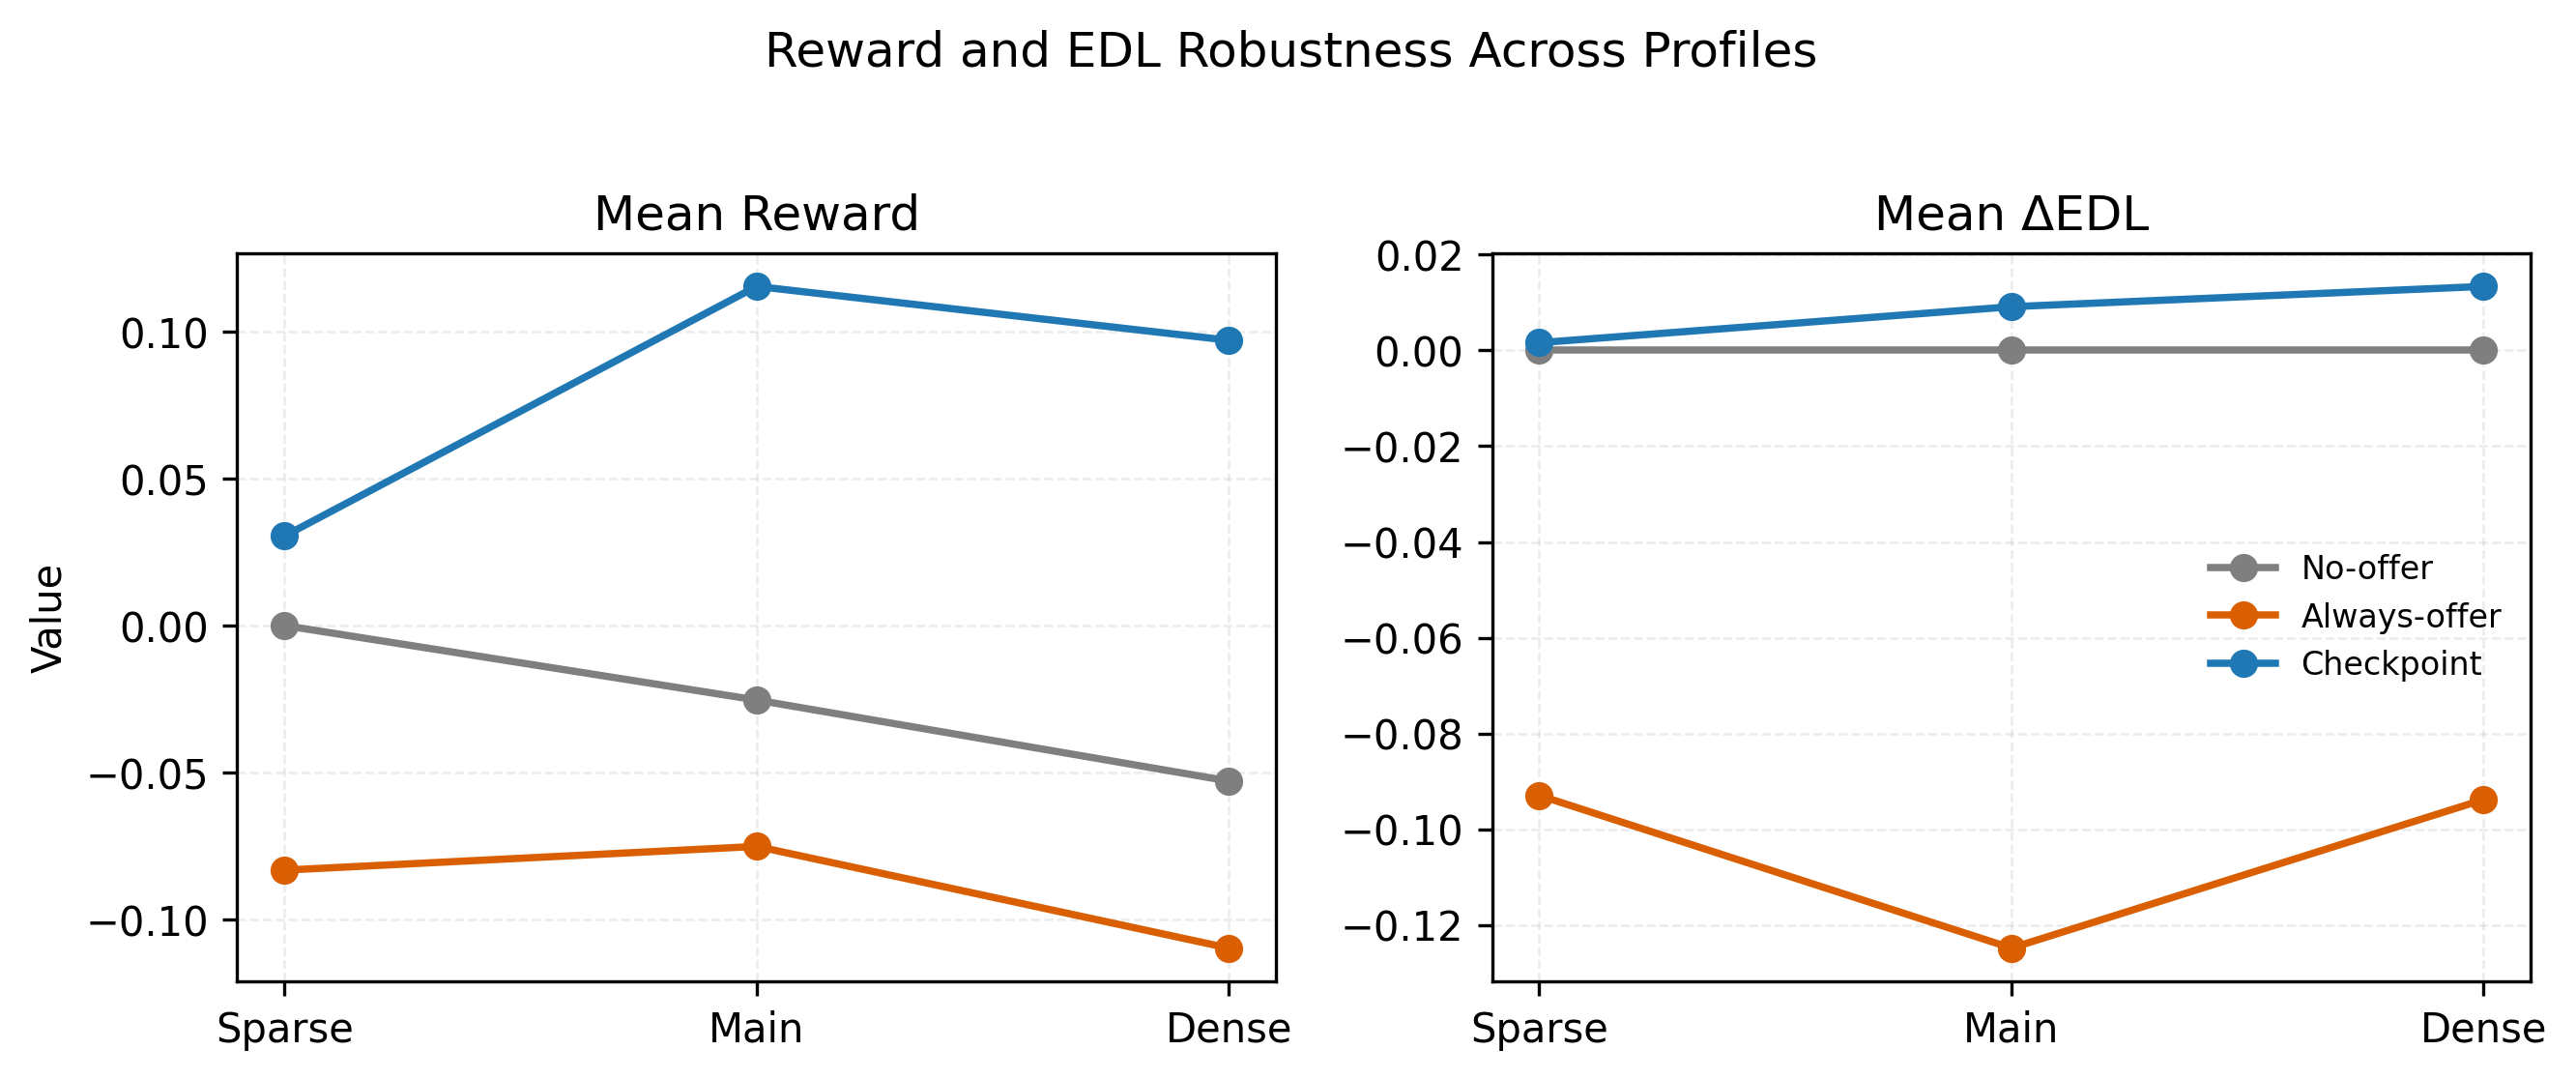
\includegraphics[width=0.9\textwidth]{figures/ch8_fig_6_8_reward_edl_robustness.png}
\caption{Reward and $\Delta EDL$ robustness across sparse/main/dense profiles.}
\label{fig:ch8_reward_edl_robustness}
\end{figure}

\begin{figure}[H]
\centering
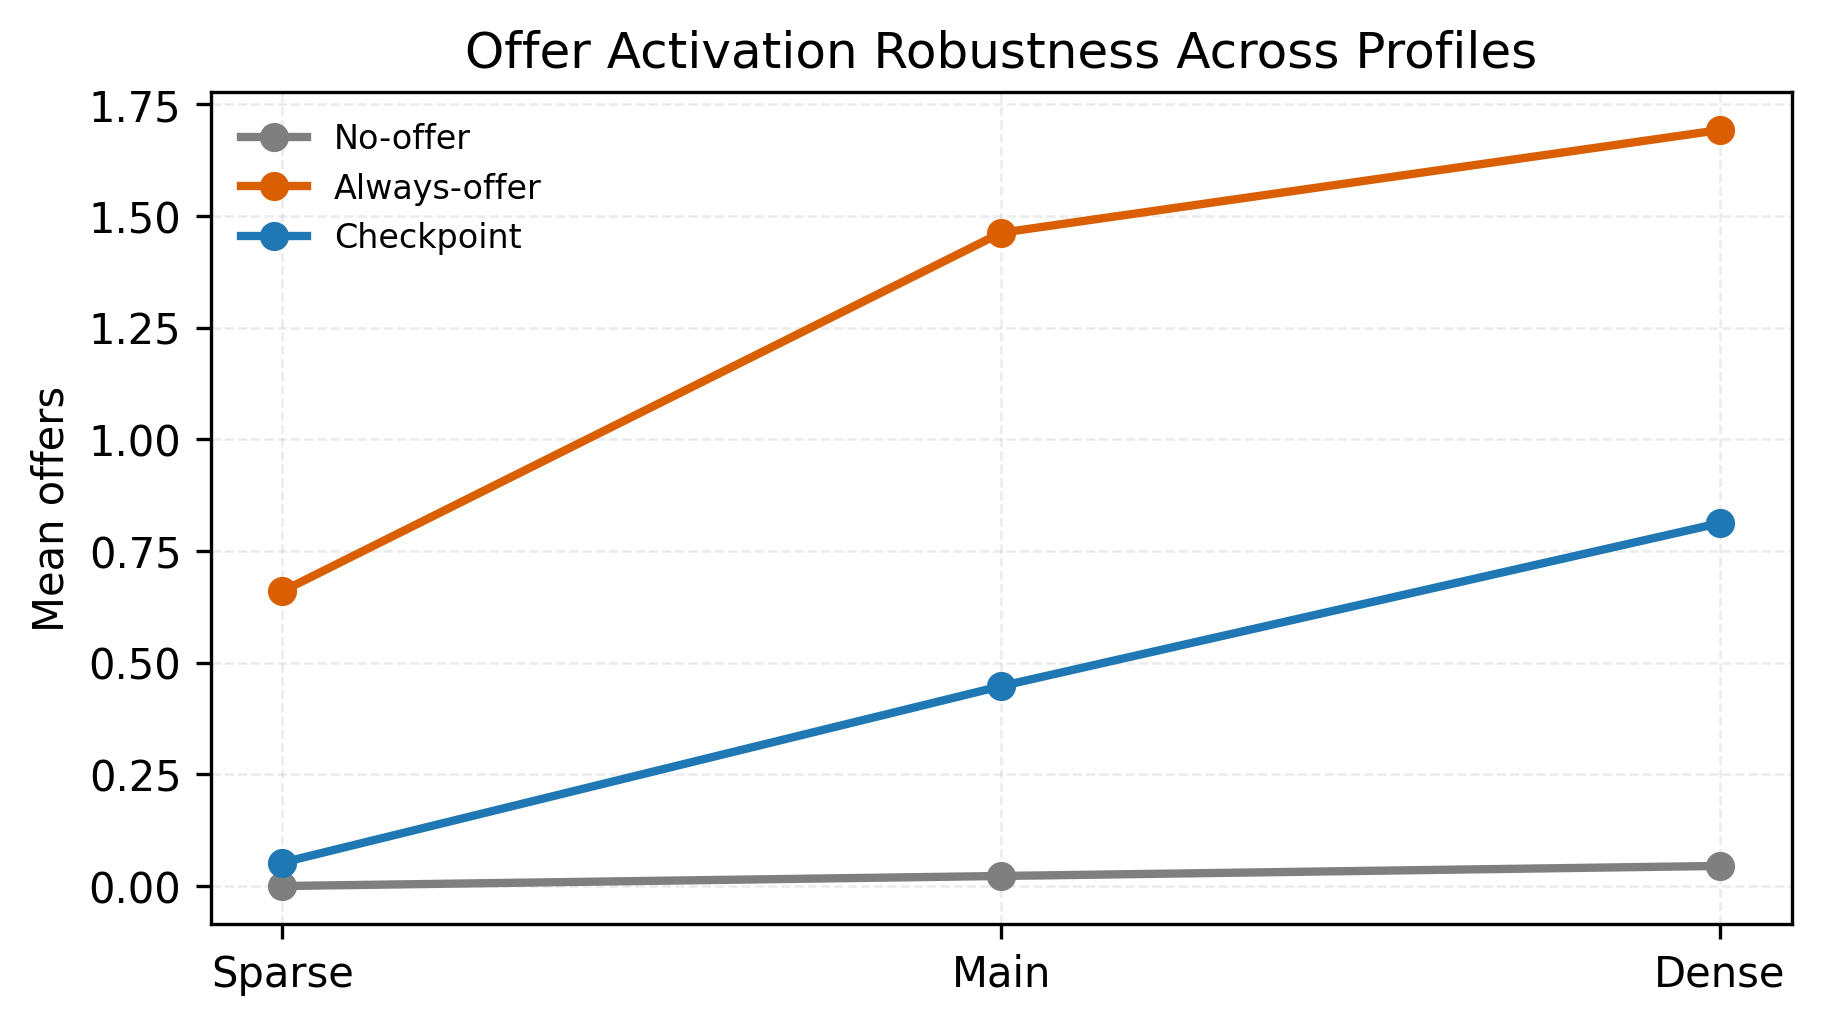
\includegraphics[width=0.9\textwidth]{figures/ch8_fig_6_9_offers_robustness.png}
\caption{Offer-activation robustness across sparse/main/dense profiles.}
\label{fig:ch8_offers_robustness}
\end{figure}

\subsection{Reward Decomposition}

To interpret policy behavior, Table~\ref{tab:ch8_reward_decomp_main} reports reward-component means under the \textit{main} profile.

\begin{table}[H]
\centering
\caption{Reward decomposition by policy in the main profile (Scenario~1).}
\label{tab:ch8_reward_decomp_main}
\begin{tabular}{lrrrr}
\toprule
Policy & Mean reward realized term & Mean reward EDL term & Mean reward accept term & Mean reward \\
\midrule
No-offer     & -0.0253 & 0.0000  & 0.0000 & -0.0253 \\
Always-offer & -0.1094 & -0.2234 & 0.3680 & -0.0752 \\
Checkpoint   & -0.0405 & 0.0949  & 0.0872 & 0.1154 \\
\bottomrule
\end{tabular}
\end{table}

The decomposition indicates that checkpoint performance is not driven by acceptance reward alone. The positive EDL component is a central contributor, and the realized-loss penalty remains materially lower than in \textit{always-offer}. Figure~\ref{fig:ch8_reward_component_breakdown} provides the signed contribution view of each reward component.

\begin{figure}[H]
\centering
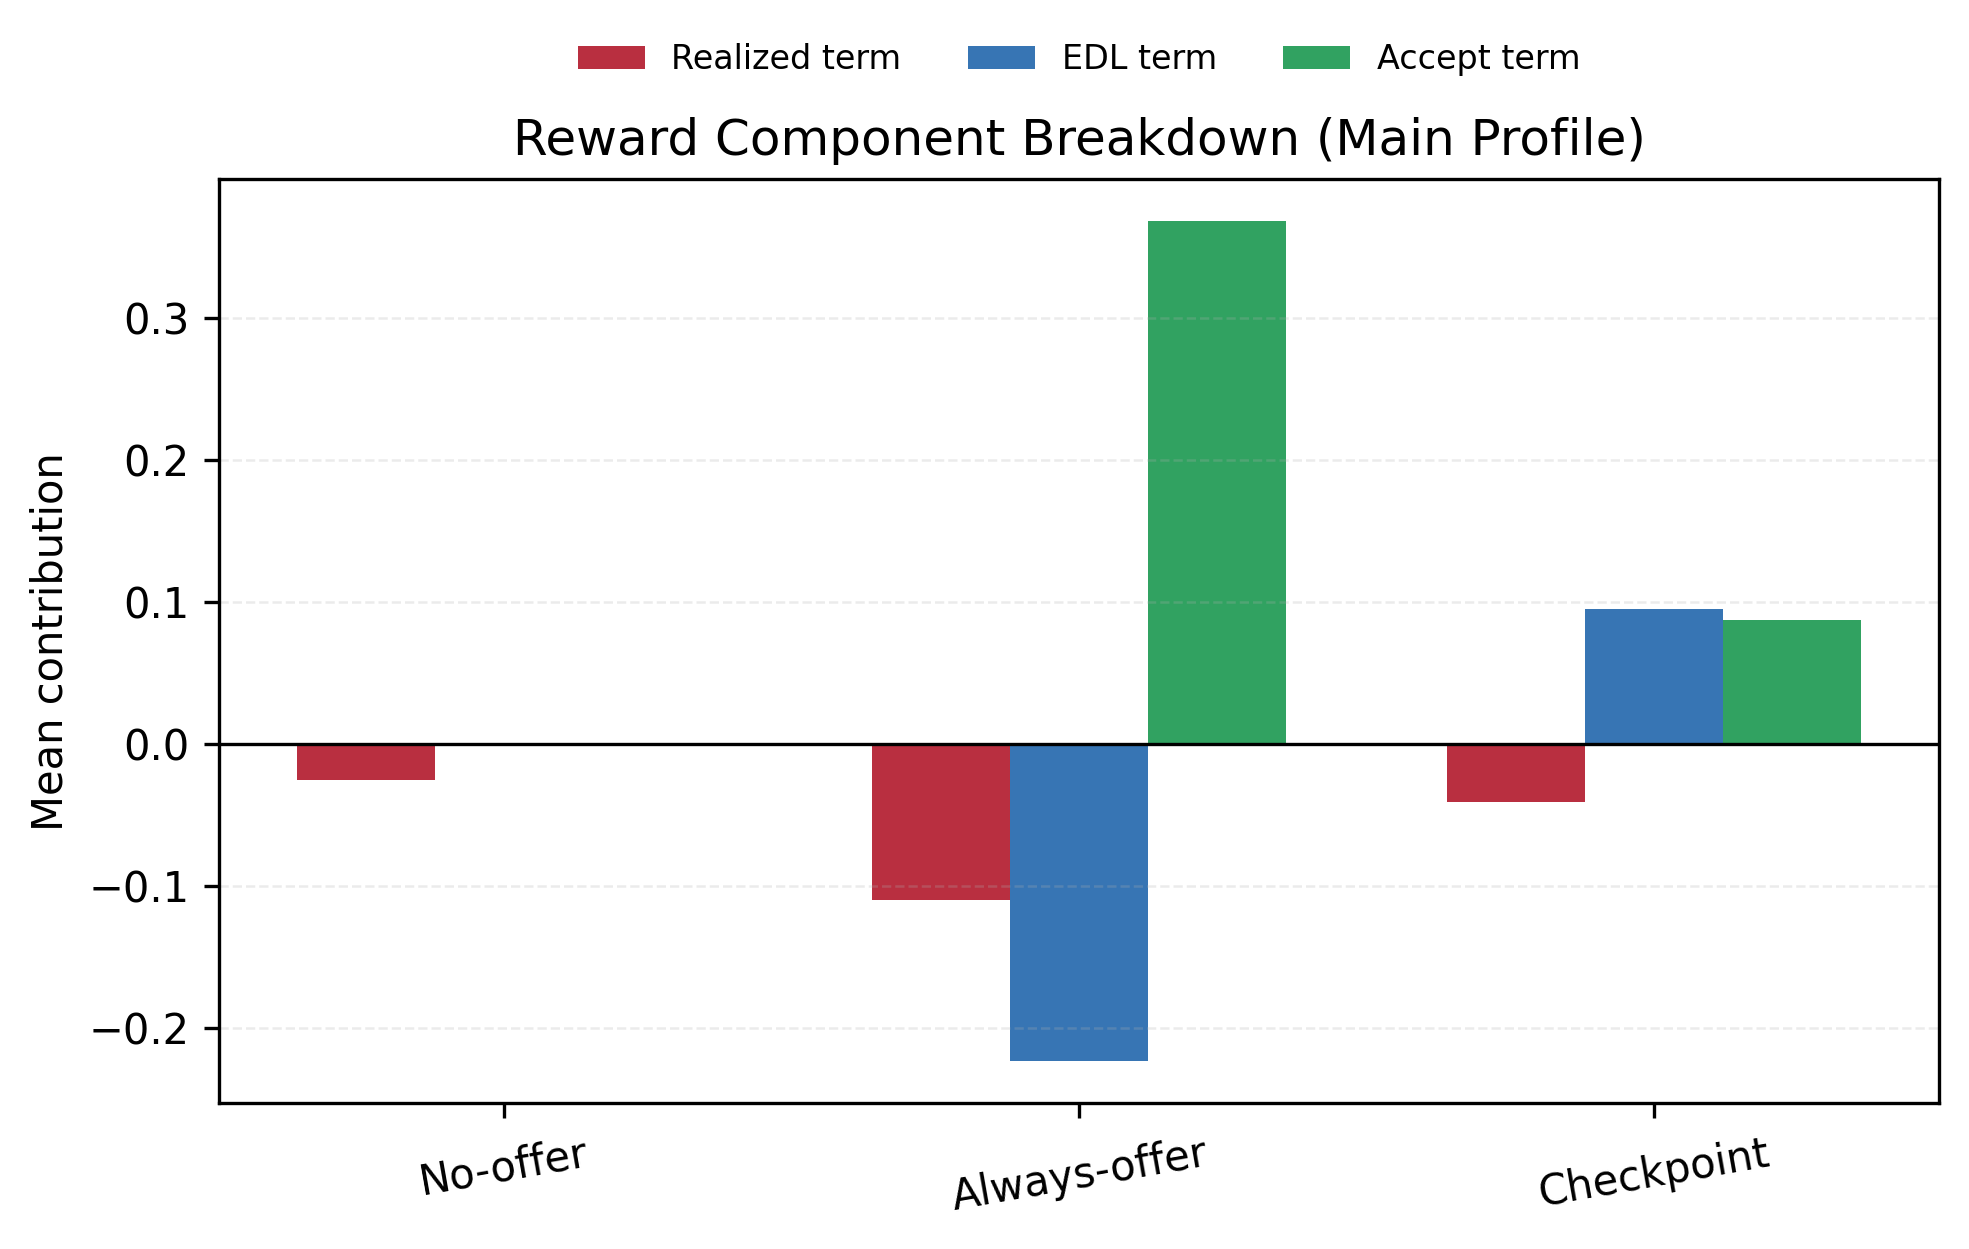
\includegraphics[width=0.9\textwidth]{figures/ch8_fig_6_10_reward_component_breakdown.png}
\caption{Main-profile reward component breakdown by policy.}
\label{fig:ch8_reward_component_breakdown}
\end{figure}

\subsection{Sensitivity Analysis (Placeholder)}

\textit{\detokenize{<TAB_6_5_S1_SENSITIVITY_MATRIX>}}

\textit{\detokenize{<FIG_6_11_S1_SENSITIVITY_RANKING>}}

\textit{This subsection reports targeted sensitivity results for reward parameters and demand-profile settings.}

\section{Scenario 2 Results}

\subsection{Training Dynamics}
\textit{\detokenize{<TAB_6_6_S2_TRAINING_SUMMARY>}}

\textit{\detokenize{<FIG_6_12_S2_TRAINING_CURVES>}}

\subsection{Main-Profile Policy Comparison}
\textit{\detokenize{<TAB_6_7_S2_MAIN_POLICY_COMPARISON>}}

\textit{\detokenize{<FIG_6_13_S2_OPTION_ACTION_DISTRIBUTION>}}

\subsection{Robustness Across Profiles}
\textit{\detokenize{<TAB_6_8_S2_ROBUSTNESS_PROFILES>}}

\textit{\detokenize{<FIG_6_14_S2_ROBUSTNESS_REWARD_EDL>}}

\subsection{Reward Decomposition and Operational Interpretation}
\textit{\detokenize{<TAB_6_9_S2_REWARD_DECOMPOSITION>}}

\textit{\detokenize{<FIG_6_15_S2_REWARD_COMPONENT_BREAKDOWN>}}

\subsection{Sensitivity Analysis}
\textit{\detokenize{<TAB_6_10_S2_SENSITIVITY_MATRIX>}}

\textit{\detokenize{<FIG_6_16_S2_SENSITIVITY_RANKING>}}

\section{Cross-Scenario Comparison}

Cross-scenario comparison follows an aligned metric schema so that Scenario~1 and Scenario~2 can be interpreted under the same operational and reward dimensions.

\begin{table}[H]
\centering
\caption{Cross-scenario comparison structure (aligned schema).}
\label{tab:ch8_cross_scenario}
\begin{tabular}{lcc}
\toprule
Dimension & Scenario~1 & Scenario~2 \\
\midrule
Action space & Binary offer activation & \texttt{\detokenize{<S2_ACTION_SPACE_DESC>}} \\
Training results & Reported & \texttt{\detokenize{<S2_TRAINING_STATUS_TOKEN>}} \\
Main-profile evaluation & Reported & \texttt{\detokenize{<S2_MAIN_EVAL_STATUS_TOKEN>}} \\
Robustness evaluation & Reported & \texttt{\detokenize{<S2_ROBUSTNESS_STATUS_TOKEN>}} \\
Sensitivity evaluation & \texttt{\detokenize{<S1_SENS_STATUS_TOKEN>}} & \texttt{\detokenize{<S2_SENS_STATUS_TOKEN>}} \\
\bottomrule
\end{tabular}
\end{table}

\textbf{Figure placeholder (position reserved):}
\begin{itemize}
\item \texttt{\detokenize{<FIG_6_17_CROSS_SCENARIO_COMPARISON>}}
\end{itemize}

\section{Findings Mapped to Research Questions}

\subsection*{RQ1: Execution mismatch identification}
The results confirm that downstream execution policies produce distinct outcomes even with fixed OR outputs. This supports the relevance of the planning-execution mismatch studied in this thesis.

\subsection*{RQ2: Decision-mechanism design}
The Scenario~1 binary refinement mechanism is operationally feasible and produces stable comparative outputs under unified evaluation settings.

\subsection*{RQ3: Comparative performance}
Across sparse/main/dense profiles, checkpoint consistently dominates \textit{always-offer} in reward and EDL direction while maintaining comparable service rate, indicating that selective activation is preferable to unconditional activation in the current setup.

\section{Chapter Summary}

This chapter reports results using one unified protocol across two scenarios, three policies, and three demand profiles. Scenario~1 numerical evidence is provided through consistent table-based reporting, and Scenario~2 uses aligned placeholders to preserve full structural comparability for direct result insertion in the next revision.

\textbf{Figure placeholder (position reserved):}
\begin{itemize}
\item \texttt{\detokenize{<FIG_6_18_CHAPTER_KEY_FINDINGS_SNAPSHOT>}}
\end{itemize}
